\chapter{Anforderungen an eine modulare und erweiterbare Bildverarbeitungssoftware}\label{anforderungen}
\addthumb{Anforderungen an das zu entwickelnde Programm}{\huge{\textbf{\thechapter.}}}{white}{haw_rot} 

%\section{Anforderungen an eine modulare und erweiterbare Bildverarbeitungssoftware}\label{einleitung:anforderungen}
\section{Einführung}
%Die Software soll grundsätzlich sowohl die Eigenschaften der Modularität, als auch der Erweiterbarkeit besitzen. Die Architektur soll offen für Weiterentwicklungen des Grundsystems sein, damit %neue Funktionen leicht eingebaut werden können. Die Variabilität der Software durch Hilfe von Erweiterungen ist wichtig für Lehre und Forschung, um in der Versuchsdurchführung möglichst %uneingeschränkt im Bereich der Software zu sein. Bei Bedarf kann eine individueller Ansatz implementiert und in das Programm integriert werden.\\

In diesem Kapitel werden die Anforderungen an eine modulare und erweiterbare Bildverarbeitungssoftware gezeigt. In mehreren Besprechungen der Stakeholder\footnote{Ein Stakeholder beschreibt einen Teilnehmer eines Projektes.} wurden die Anforderungen ermittelt. Diese werden in die beiden Bereiche \textit{Nichtfunktionale Anforderungen} und \textit{Funktionale Anforderungen} eingeteilt. Nach einer Evaluierung bestehender Anwendungen wird entschieden, ob eine eigene Software implementiert werden soll.


\section{Nichtfunktionale Anforderungen}

Nach Balzert \cite[9]{balzert:swa} beschreiben nichtfunktionale Anforderungen, \textit{wie} ein System arbeitet. Sie üben besonderen Einfluss auf die Softwarearchitektur eines Systems aus.
Während der Besprechungen konnten folgende nichtfunktionale Anforderungen ermittelt werden.

\begin{itemize}
\item  \textbf{Modularer Aufbau des Systems}(1)\\
	  Die Software soll in den Grundfunktionen erweiterbar sein, die nach einem neuen Build-Prozess zur Verfügung stehen. So soll es möglich sein, neue Bedienelemente der Benutzeroberfläche und neue Funktionen der Anwendung hinzuzufügen.
	  
\item \textbf{Erweiterbarkeit durch den Anwender}(2)\\
	Anwender sollen die Möglichkeit haben, das Programm mit selbst programmierten Algorithmen und Plug-ins zu erweitern. Die eigene Implementierung von Bildverarbeitungsprozessen ist essentiell im Bereich der Lehre.
	
\item \textbf{Die Programmiersprache Java}(3)\\
	Die Studierenden des Studiengangs sollen im Modul \glqq medizinische Bildverarbeitung\grqq\ Ihre Kompetenzen im Bereich der Programmierung mit Java erweitern. Dadurch soll die Anwendung in Java umgesetzt und erweiterbar sein.
	
\item \textbf{Externe Bildverarbeitungsbibliotheken}(4)\\
	Algorithmen in der Bildverarbeitung sind oft komplex und umfangreich. Nicht jeder benötigte Verarbeitungsprozess eignet sich zum selbst implementieren (sowohl im Lehr- als auch Forschungsbereich). Durch den Einsatz von Bibliotheken wird ein grundlegender Satz an Algorithmen vorgegeben, auf den der Benutzer zurückgreifen und in den Plug-ins verwenden kann.
	
\item \textbf{Verarbeitung medizinische Daten mit Hilfe des DICOM-Standards}(5)\\
	Medizinische Bilddaten besitzen neben den rohen Pixeldaten noch eine Vielzahl zusätzlicher Information, wie Patientendaten oder Seriennummern der Aufnahmen und benötigen eine spezielle Verarbeitung. Anders als übliche Grauwertbilder besitzen DICOM-Daten unter Anderem nicht 255 sondern bis zu $2^{16}$ verschiedene Grauwerte.
\end{itemize}

\section{Funktionale Anforderungen}

Diese Art der Anforderungen legen fest, \textit{was} das Programm leisten soll und bestimmen Funktionen und Verhalten \cite[9]{balzert:swa}. Sie überschneiden sich oder stehen in Beziehung zu den nichtfunktionalen Anforderungen.

\begin{itemize}
\item \textbf{Dynamische Parameterübergabe bei einer Plug-in-Ausführung}(6)\\
		Aus der Anwendererweiterbarkeit ergibt sich eine funktionale Anforderung. Nicht immer können alle Eigenschaften und Werte der Algorithmen während der Implementierung vom Anwender bestimmt werden. Durch die Abhängigkeit von den zu bearbeitenden Bilddaten und Algorithmen muss die Möglichkeit geboten werden, Parameter während der Laufzeit der Anwendung zu bestimmen.

\item \textbf{Manuelle Auswahl signifikanter Punkte zur Verarbeitung in Plug-ins}(7)\\
		Zusätzlich zu den dynamischen Parametern müssen einzelne Bildpunkte interaktiv vom Benutzer ausgewählt und später von Algorithmen benutzt werden können. Manche Bildverarbeitungsprozesse benötigen beispielsweise sogenannte Saatpunkte die von Anwender manuell ausgewählt werden müssen.

\item \textbf{Anwendung der Algorithmen im dreidimensionalen Raum}(8)\\
	  Eine Vielzahl an Bildaufnahmen liegen als dreidimensionaler Datensatz vor. Eine Bildreihe muss folglich zusätzlich zur xy-Ebene auch in z-Richtung zu bearbeiten sein.

\item \textbf{Darstellung mehrerer Bilddatensätze(9)}\\
	Das Programm soll mehrere dreidimensionale Bildreihen zur selben Zeit in verschiedenen Fenstern anzeigen können. Das erlaubt den Benutzern die Datensätze in Beziehung zueinander zu betrachten.

\item \textbf{Darstellung aller Bildebenen}(10)\\
	  Ein dreidimensionaler Datensatz macht es möglich, nicht nur die Bilder der xy-Ebene (Axial) sondern auch die xz-(Coronal) sowie yz-Ebene(Sagittal) darzustellen. Zwischen den Ansichten soll der Benutzer wechseln können.

\item \textbf{Dynamische Anzeige eines Punktes in allen Bildebenen}(11)\\
	  Sind drei gleiche Datensätze in drei verschiedenen Fenstern geöffnet sollen diese dynamisch reagieren, wenn der Benutzer einen Punkt eines Datensatzes auswählt. Angenommen ein Datensatz ist in axialer, coronaler und sagittaler Ansicht geöffnet. Wählt der Nutzer einen Bildpunkt aus der axialen Ansicht, sollen die beiden übrigen geöffneten Fenter aktualisiert werden und den gleichen Punkt in ihrer jeweiligen Ansicht referenzieren.
	  
\item \textbf{Anzeige der dreidimensionalen Datensätze in $(x, y, z)$} (12)\\
	 Damit die Darstellung der verschiedenen Ebenen möglich wird, muss der gesamte dreidimensionale Datensatz zur Anzeige zur Verfügung stehen. Der Anwender soll durch die einzelnen Schichten der Bildreihen scrollen können.
\end{itemize}
%\footnotetext{http://www.radiantviewer.com/de/}

% Jetzt eine gleitende Abbildung, die Abbildung wird am oberen 
% Seitenrand positioniert, die Fußnote erhält die Nummer 3
% Der Fußnotenbefehl wird nochmal geschützt

\section{Evaluierung bestehender Software}

Frei verfügbare Software im medizinischen Bereich beschränkt sich oft die vorgegebenen Funktionen des Programms und bietet keine Möglichkeiten der Erweiterung. Zusätzlich liegt der Fokus auf der Darstellung der Patientenbilder und weniger an den Algorithmen zur Bildverarbeitung. Abbildung \ref{radiant} zeigt den Screenshot des DicomViewers RadiAnt\footnote{http://www.radiantviewer.com/de/}. Die Bilder können einzeln, oder wie auf dem Bild zu sehen, im Bezug zueinander betrachtet werden. Die Werkzeugleiste oben ermöglicht die für DICOM-Bilder typischen Operationen.
Zwar gibt es auf dem Markt auch Open-Source Lösungen mit Schwerpunkt auf Bildverarbeitung, jedoch eigenen sich diese nur bedingt für den Einsatz in der Lehre. Die Programme bieten eine Vielzahl an Funktionen, allerdings benötigt die Entwicklung von Erweiterungen einen erheblichen Zeitaufwand.
 
\begin{figure}[htbp]
  \vspace{0.5cm}
  \centering
  \fbox{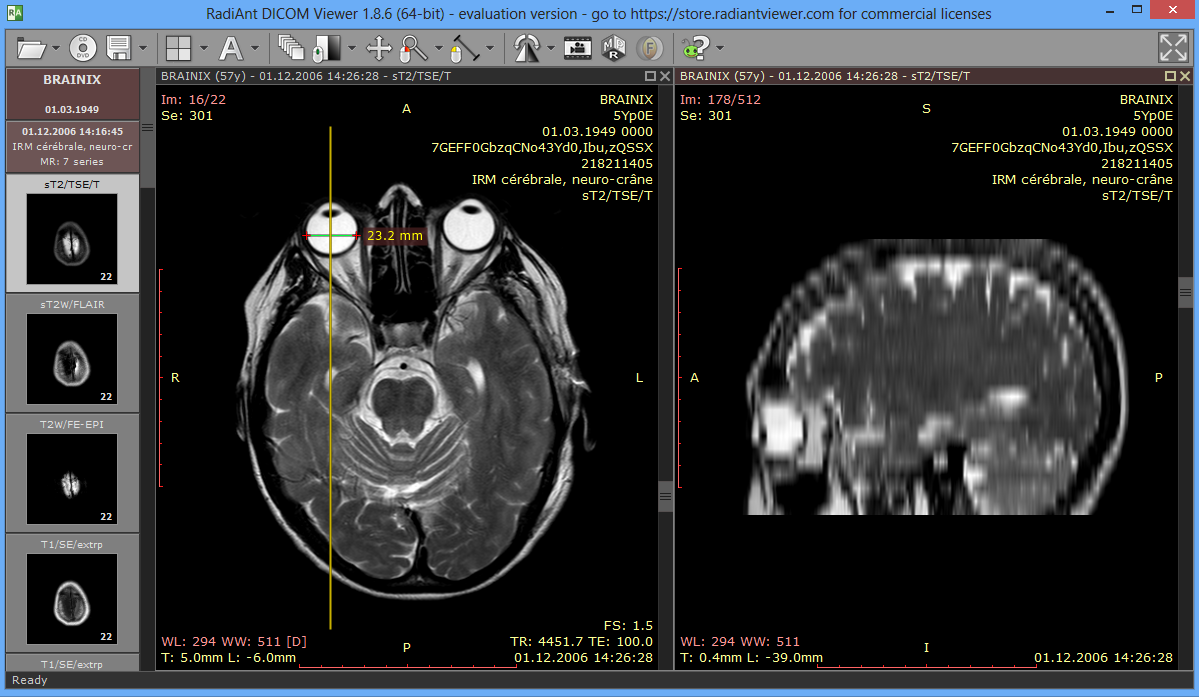
\includegraphics[angle=0,width=9cm]{./img/RadiAnt.png}}
   \caption{RadiAnt - DicomViewer}
  \label{radiant}
  \vspace{0.5cm}
\end{figure}


\section{Slicer 3D}

Slicer 3D\footnote{http://www.slicer.org} (Abbildung \ref{slicer3d}) ist ein umfassendes Werkzeug für die medizinische Bildverarbeitung im zwei- und dreidimensionalen Raum. Die quelloffene Software bietet Möglichkeiten eigene Erweiterungen zu implementieren. Slicer verwendet als Bibliotheken unter anderem das Insight Toolkit und das Visualization Toolkit\footnote{Insight Toolkit(ITK) und Visualization Toolkit (VTK) sind umfassende in C++ entwickelte Programmbibliotheken zur medizinischen Bildverarbeitung und Visualisierung.}. Die Erweiterungen werden in Python implementiert und dienen zur Anwendung der Bildverarbeitungsalgorithmen. Es fehlt die Möglichkeit der modularen Erweiterung bezüglich neuer Funktionen. Das Labor setzt in naher Zukunft ein PACS ein und die Software soll Möglichkeiten bieten, dieses System später zu integrieren, um DICOM-Daten über das Netzwerk zu beziehen.
%Das Modul \glqq medizinische Bildverarbeitung\grqq\ baut auf der Programmiersprache Java auf und ist eine weitere Voraussetzung für einen Einsatz im Lehrgebiet. Module in Slicer werden in Python %implementiert. Die Studierenden müssten damit eine zusätzliche Sprache lernen.\\

\begin{figure}[htbp]
  \vspace{0.5cm}
  \centering
  \fbox{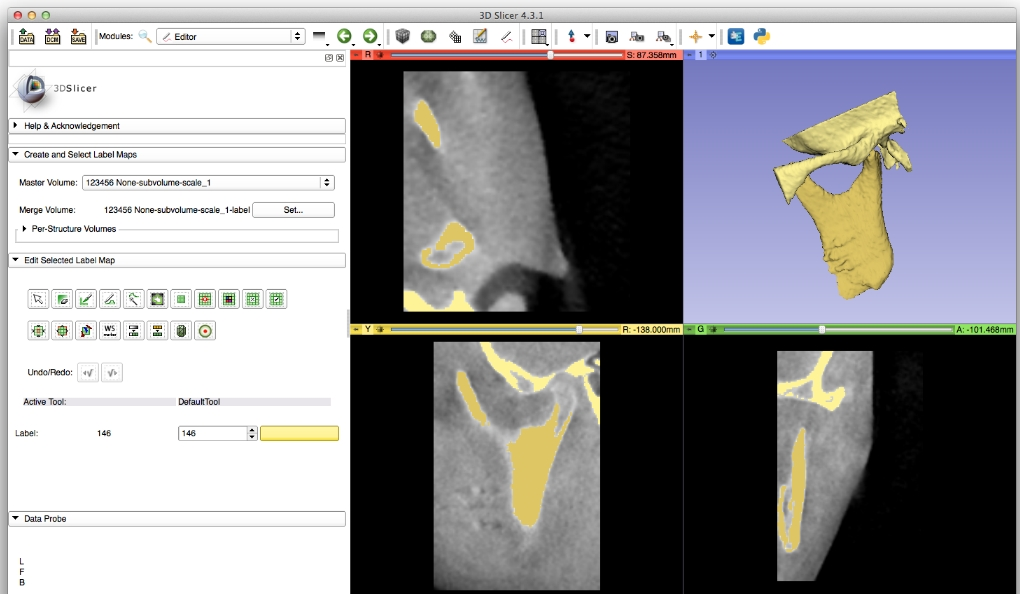
\includegraphics[angle=0,width=9cm]{./img/Screenshot-3DSlicer.png}}
  \floatfoot{Quelle: http://www.linuxlinks.com/portal/content/reviews/Health/Screenshot-3DSlicer.png - abgerufen am 11.01.2014}
  \caption{Screenshot Slicer 3D}
  \label{slicer3d}
  \vspace{0.5cm}
\end{figure}

\section{ImageJ}

ImageJ ist \glqq State Of The Art\grqq\ im Bereich der Bildverarbeitung in Java\footnote{http://rsbweb.nih.gov/ij/}). Im Grundzustand liefert ImageJ die Standardfunktionen der Bildverarbeitung wie Abbildung \ref{imagej} zeigt. Unter Anderem kann das Bildmaterial analysiert oder mit Filtern bearbeitet werden. ImageJ verarbeitet sowohl Grauwertbilder als auch Farbbilder in den gängigen Formaten wie PNG, JPEG und vielen Anderen. Mit Hilfe der \glqq ImageStacks\grqq\ ist auch eine Bearbeitung im dreidimensionalen Bildraum möglich. Erweiterungen können schnell und zielgerichtet entwickelt werden. Im Modul \glqq Bildverarbeitung\grqq\ der Fakultät Informatik wird ImageJ als Standard zum Bearbeiten der Übungsaufgaben verwendet. Für einen Einsatz im Studiengang Biomedizinische Technik fehlt allerdings die grundlegende Unterstützung von medizinischen Bilddaten im DICOM-Format. Die Funktionalität lässt sich über Plug-ins nachträglich hinzufügen, allerdings fehlt eine Bibliothek die bereits implementierte Algorithmen zur Verfügung stellt, sowie eine Verknüpfung von ImageJ-Klassen wie FloatProcessor oder ByteProcessor in Bildformate der Bibliotheken.

\begin{figure}[htbp]
  \vspace{0.5cm}
  \centering
  \fbox{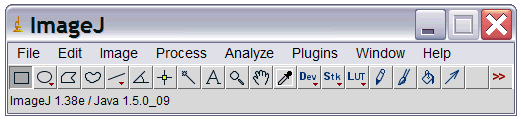
\includegraphics[angle=0,width=9cm]{./img/imagej-window.png}}
  \caption{Die Benutzeroberfläche von ImageJ}
  \floatfoot{ Quelle:  http://rsbweb.nih.gov/ij/features.html - abgerufen am 11.01.2014}
  \label{imagej}
  \vspace{0.5cm}
\end{figure}

\begin{comment}
\section{Anforderungen}

Für eine Software die an der Hochschule Landshut für Lehre sowie Forschung im Bereich der medizinischen Bildverarbeitung eingesetzt werden kann ergeben sich folgende Anforderungen:

\begin{itemize}
\item \textbf{Erweiterbarkeit durch den Anwender} \\
	  Anwender sollen die Möglichkeit haben, das Programm mit selbst programmierten Algorithmen zu erweitern. Die eigene Implementierung von Bildverarbeitungsprozessen ist essentiell im Bereich der Lehre.
	  
\item \textbf{Interaktive Benutzereingaben}
	  Aus der Anwendererweiterbarkeit ergibt sich eine weitere Anforderung. Nicht immer können alle Eigenschaften und Werte der Algorithmen während der Implementierung vom Anwender bestimmt werden. Durch die Abhängigkeit von Bilddaten zu Algorithmen muss die Möglichkeit geboten werden, Parameter während der Laufzeit der Anwendung zu bestimmen. Zusätzlich müssen einzelne Bildpunkte interaktiv vom Benutzer ausgewählt und später von Algorithmen benutzt werden können.

\item \textbf{Anwendung der Algorithmen im dreidimensionalen Raum}\\
	  Eine Vielzahl an Bildaufnahmen liegen als dreidimensionaler Datensatz vor. Eine Reihe von Bildern muss folglich zusätzlich zur xy-Ebene auch in z-Richtung zu bearbeiten sein.

\item \textbf{Darstellung aller Ebenen der Bilddaten}\\
	  Ein dreidimensionaler Datensatz macht es möglich, nicht nur die Bilder der xy-Ebene sondern auch die xz- sowie yz-Ebene darzustellen. Es soll möglich sein, in einem Bildsatz einen Punkt auszuwählen und in Darstellungen mit anderer Ebenenansicht der gleichen Daten anzeigen.
	
\item \textbf{Modularer Aufbau} \\
	  Die Software soll auch in den Grundfunktionen erweiterbar sein, die bei Auslieferung des Programms sofort zur Verfügung stehen (Skalierung, Rotation, etc.). Anders als die von Benutzern erstellten Plug-ins, die abhängig vom Anwender sind, muss eine Möglichkeit zur globalen Erweiterung gegeben werden.

\item \textbf{Unterstützung des Dicom-Standards}\\
	  Medizinische Bilddaten besitzen neben den rohen Pixeldaten noch eine Vielzahl zusätzlicher Information wie Patientendaten oder Seriennummern der Aufnahmen und benötigen eine spezielle Verarbeitung. Anders als übliche Grauwertbilder besitzen DICOM-Daten unter Anderem nicht 255 sondern bis zu $2^{16}$ verschiedene Grauwerte.
	  
\item \textbf{Implementierung in der Programmiersprache Java}\\
	  Das Modul zur Bildverarbeitung der Biomedizinischen Technik findet in Java statt. Dadurch wird die Programmiersprache eine Anforderung, da ein Einsatz für die Lehre sonst nur erschwert möglich ist.

\item \textbf{Grundausstattung an medizinischen Bibliotheken}\\
	  Algorithmen in der Bildverarbeitung sind oft komplex und umfangreich. Nicht jeder benötigte Verarbeitungsprozess eignet sich zum selbst implementieren (Sowohl im Lehr- als auch Forschungsbereich). Durch den Einsatz von Bibliotheken wird ein grundlegender Satz an Algorithmen vorgegeben, auf den der Benutzer zurückgreifen und in den Plug-ins verwenden kann.
\end{itemize} 
\end{comment}

\section{Ein Vergleich der verfügbaren Anwendung mit den Anforderungen der Stakeholder}

\begin{table}
    \begin{tabularx}{\textwidth}{|p{7cm}|X|X|X|}
    \toprule
    \hline
    			         							& \textbf{RadiAnt}     								 & \textbf{Slicer3D} 									 & \textbf{ImageJ}\\ \hline
    modularer Aufbau (1)		 					& 
\includegraphics[width=0.5cm]{./img/no.pdf}	 & 
\includegraphics[width=0.5cm]{./img/no.pdf}  & 
\includegraphics[width=0.5cm]{./img/yes.pdf} \\ \hline
    Java (3)	 									& 
\includegraphics[width=0.5cm]{./img/no.pdf}	 & 
\includegraphics[width=0.5cm]{./img/no.pdf}  & 
\includegraphics[width=0.5cm]{./img/yes.pdf}\\ \hline
    multiple Datensätze anzeigen (9)				& 
\includegraphics[width=0.5cm]{./img/yes.pdf} & 
\includegraphics[width=0.5cm]{./img/yes.pdf} & 
\includegraphics[width=0.5cm]{./img/yes.pdf} \\ \hline
    Bildanzeige in $(x, y, z)$ (12)					& 
\includegraphics[width=0.5cm]{./img/yes.pdf} & 
\includegraphics[width=0.5cm]{./img/yes.pdf} &  
\includegraphics[width=0.5cm]{./img/yes.pdf}\\ \hline
    Ansicht der Ebenen  $(xy, xz, yz)$ (10)			& 
\includegraphics[width=0.5cm]{./img/yes.pdf} & 
\includegraphics[width=0.5cm]{./img/yes.pdf} & 
\includegraphics[width=0.5cm]{./img/no.pdf} \\ \hline
    Dynamische Anzeige der Punkte(11)	&
\includegraphics[width=0.5cm]{./img/yes.pdf} & 
\includegraphics[width=0.5cm]{./img/yes.pdf}  & 
\includegraphics[width=0.5cm]{./img/no.pdf}\\ \hline
    DICOM (5)									    & 
\includegraphics[width=0.5cm]{./img/yes.pdf}	& 
\includegraphics[width=0.5cm]{./img/yes.pdf}	& 
\includegraphics[width=0.5cm]{./img/no.pdf}\\ \hline	
    Plug-ins (2)		 							& 
\includegraphics[width=0.5cm]{./img/no.pdf}	& 
\includegraphics[width=0.5cm]{./img/yes.pdf} 	& 
\includegraphics[width=0.5cm]{./img/yes.pdf}  \\ \hline
    Bibliotheken zur Bildverarbeitung (4)		 	& n.A.			& 
\includegraphics[width=0.5cm]{./img/yes.pdf}  		  		& 
\includegraphics[width=0.5cm]{./img/no.pdf}  \\ \hline
    Dynamische Parameter (6)						& n.A.				& 
\includegraphics[width=0.5cm]{./img/yes.pdf}  		  		& 
\includegraphics[width=0.5cm]{./img/yes.pdf}  \\ \hline
    Manuelle Punktauswahl (7)		 				& n.A.				& 
\includegraphics[width=0.5cm]{./img/yes.pdf}		  		& 
\includegraphics[width=0.5cm]{./img/yes.pdf} \\ \hline
    Algorithmen in $(x, y, z)$ (8)					& n.A.& 
\includegraphics[width=0.5cm]{./img/yes.pdf}  &  
\includegraphics[width=0.5cm]{./img/yes.pdf} \\ \hline
    
    \bottomrule
    \end{tabularx}
    \caption {Gegenüberstellung der Anforderungen und verfügbarer freier Software}
    \label{table:anforderungen}
\end{table}

Tabelle \ref{table:anforderungen} zeigt eine Gegenüberstellung der evaluierten Software zu den Anforderungen. Slicer3D und ImageJ erfüllen einen hohen Grad davon, allerdings fehlen wichtige sogenannte harte\footnote{Es wird zwischen harten und weichen Anforderungen unterschieden. Harte Anforderungen müssen erfüllt werden, während Weiche erfüllt werden können \cite[9]{balzert:swa}} Anforderungen. Slicer3D lässt einen einfachen Ansatz zur modularen Erweiterung der Benutzeroberfläche und Anwendungsfunktionen vermissen. ImageJ hingegen bietet diese Variabilität. Allerdings ist die Verarbeitung von DICOM-Daten nur über ein Plug-in möglich und es fehlt eine Grundlage in Algorithmen zur medizinischen Bildverarbeitung. Zusätzlich zu den vorgestellten Anwendungen bietet auch MatLab\footnote{http://www.mathworks.de/products/matlab/} umfangreiche Bildverarbeitungskomponenten, unter anderem auch zur Verarbeitung von DICOM-Objekten an. Die hohen Lizenzkosten sprechen allerdings deutlich gegen einen Einsatz in der Lehre, da Anwendungen nur auf begrenzt vielen Maschinen installiert werden können und dadurch die Zahl der Arbeitsplätze für Studierende erheblich unnötig eingeschränkt ist. Aufgaben können nur im Labor bearbeitet werden, was voraussetzt, dass das Labor zu jeder Zeit geöffnet werden muss.
Da in den vorgestellten Anwendungen keine Lösung verfügbar ist, die alle Voraussetzungen erfüllt, soll eine Software entwickelt werden, die für das Labor für medizinische Bildverarbeitung, Algorithmen und Krankenhaus IT die benötigten funktionalen und nichtfunktionalen Anforderungen erfüllt.